\documentclass[hidelinks]{article}
\usepackage[english]{babel} 
\usepackage[utf8x]{inputenc}
%% Hyperlinks 
\usepackage{hyperref}
\hypersetup{
    colorlinks,
    linkcolor={red!50!black},
    citecolor={blue!50!black},
    linktoc=all,
    urlcolor={blue!80!black}
}
%% Graphics
\usepackage{graphicx}
\usepackage{float}

\usepackage{enumerate}
\usepackage{multicol}
% Math packages
\usepackage{amsmath}
\usepackage{amssymb}

% Algorithms
\usepackage{algorithm}
\usepackage[noend]{algpseudocode}
\newcommand\Let[2]{\State #1 $\gets$ #2}
\algrenewcomment[1]{\(\qquad \triangleright\) #1}
\newcommand\Blet[2]{\State \textbf{let} #1 \textbf{be} #2}
\errorcontextlines\maxdimen
% begin vertical rule patch for algorithmicx
% borrowing from http://tex.stackexchange.com/questions/41956/marking-conditional-versions-with-line-in-margin
% see http://tex.stackexchange.com/questions/110431/ploblems-with-vertical-lines-in-algorithmicx
\RequirePackage{zref-abspage}
\RequirePackage{zref-user}
\RequirePackage{tikz}
%\RequirePackage{atbegshi}
%\usetikzlibrary{calc}
\RequirePackage{tikzpagenodes}
\RequirePackage{etoolbox}
\makeatletter
\newcommand*\ALG@lastblockb{b}
\newcommand*\ALG@lastblocke{e}
\apptocmd{\ALG@beginblock}{%
    %\typeout{beginning block, nesting level \theALG@nested, line \arabic{ALG@line}}%
    \ifx\ALG@lastblock\ALG@lastblockb
        \ifnum\theALG@nested>1\relax\expandafter\@firstoftwo\else\expandafter\@secondoftwo\fi{\ALG@tikzborder}{}%
    \fi
    \let\ALG@lastblock\ALG@lastblockb%
}{}{\errmessage{failed to patch}}

\pretocmd{\ALG@endblock}{%
    %\typeout{ending block, nesting level \theALG@nested, line \arabic{ALG@line}}%
    \ifx\ALG@lastblock\ALG@lastblocke
        \addtocounter{ALG@nested}{1}%
        \addtolength\ALG@tlm{\csname ALG@ind@\theALG@nested\endcsname}%
        \ifnum\theALG@nested>1\relax\expandafter\@firstoftwo\else\expandafter\@secondoftwo\fi{\endALG@tikzborder}{}%
        \addtolength\ALG@tlm{-\csname ALG@ind@\theALG@nested\endcsname}%
        \addtocounter{ALG@nested}{-1}%
    \fi
    \let\ALG@lastblock\ALG@lastblocke%
}{}{\errmessage{failed to patch}}
\tikzset{ALG@tikzborder/.style={line width=0.5pt,black}}
\newcommand*\currenttextarea{current page text area}
\newcommand*{\updatecurrenttextarea}{%
    \if@twocolumn
        \if@firstcolumn
            \renewcommand*{\currenttextarea}{current page column 1 area}%
        \else
            \renewcommand*{\currenttextarea}{current page column 2 area}%
        \fi
    \else
        \renewcommand*\currenttextarea{current page text area}%
    \fi
}
\newcounter{ALG@tikzborder}
\newcounter{ALG@totaltikzborder}
\newenvironment{ALG@tikzborder}[1][]{%
    % Allow user to overwrite the used style locally
    \ifx&#1&\else
        \tikzset{ALG@tikzborder/.style={#1}}%
    \fi
    \stepcounter{ALG@totaltikzborder}%
    \expandafter\edef\csname ALG@ind@border@\theALG@nested\endcsname{\theALG@totaltikzborder}%
    \setcounter{ALG@tikzborder}{\csname ALG@ind@border@\theALG@nested\endcsname}%
    %\typeout{begin ALG border nesting level=\theALG@nested, tikzborder=\theALG@tikzborder, tlm=\the\ALG@tlm}%
    \tikz[overlay,remember picture] \coordinate (ALG@tikzborder-\theALG@tikzborder);% node {\theALG@tikzborder};% Modified \tikzmark macro
    \zlabel{ALG@tikzborder-begin-\theALG@tikzborder}%
    % Test if end-label is at the same page and draw first half of border if not, from start place to the end of the page
    \ifnum\zref@extract{ALG@tikzborder-begin-\theALG@tikzborder}{abspage}=\zref@extract{ALG@tikzborder-end-\theALG@tikzborder}{abspage} \else
        \updatecurrenttextarea
        \ALG@drawvline{[shift={(0pt,.5\ht\strutbox)}]ALG@tikzborder-\theALG@tikzborder}{\currenttextarea.south east}{\ALG@thistlm}%
        % If it spreads over more than two pages:
        \newcounter{ALG@tikzborderpages\theALG@tikzborder}%
        \setcounter{ALG@tikzborderpages\theALG@tikzborder}{\numexpr-\zref@extract{ALG@tikzborder-begin-\theALG@tikzborder}{abspage}+\zref@extract{ALG@tikzborder-end-\theALG@tikzborder}{abspage}}%
        \ifnum\value{ALG@tikzborderpages\theALG@tikzborder}>1
            \edef\nextcmd{\noexpand\AtBeginShipoutNext{\noexpand\ALG@tikzborderpage{\theALG@tikzborder}{\the\ALG@thistlm}}}%some pages need a border on the whole page
            \nextcmd
        \fi
    \fi
}{%
    \setcounter{ALG@tikzborder}{\csname ALG@ind@border@\theALG@nested\endcsname}%
    %\typeout{end ALG border nesting level=\theALG@nested, tikzborder=\theALG@tikzborder, tlm=\the\ALG@tlm}%
    \tikz[overlay,remember picture] \coordinate (ALG@tikzborder-end-\theALG@tikzborder);% node {\theALG@tikzborder};% Modified \tikzmark macro
    \zlabel{ALG@tikzborder-end-\theALG@tikzborder}%
    % Test if begin-label is at the same page and draw whole border if so, from start place to end place
    \updatecurrenttextarea
    \ifnum\zref@extract{ALG@tikzborder-begin-\theALG@tikzborder}{abspage}=\zref@extract{ALG@tikzborder-end-\theALG@tikzborder}{abspage}\relax
        \ALG@drawvline{[shift={(0pt,.5\ht\strutbox)}]ALG@tikzborder-\theALG@tikzborder}{ALG@tikzborder-end-\theALG@tikzborder}{\ALG@thistlm}%
    % Otherwise draw second half of border, from the top of the page to the end place
    \else
        %\settextarea
        \ALG@drawvline{\currenttextarea.north west}{ALG@tikzborder-end-\theALG@tikzborder}{\ALG@thistlm}%
    \fi
}
\newcommand*{\ALG@drawvline}[3]{%#1=from, #2=to, #3=value of \ALG@tlm/\ALG@thisthm
    \begin{tikzpicture}[overlay,remember picture]
        \draw [ALG@tikzborder]
            let \p0 = (\currenttextarea.north west), \p1=(#1), \p2 = (#2)
             in
            (#3+\fboxsep+.5\pgflinewidth+\x0,\y1+\fboxsep+.5\pgflinewidth)%-\fboxsep-.5\pgflinewidth
             --
            (#3+\fboxsep+.5\pgflinewidth+\x0,\y2-\fboxsep-.5\pgflinewidth)
            %node[midway,anchor=east] {\ALG@tikzbordertext}
        ;
    \end{tikzpicture}%
}
\newcommand{\ALG@tikzborderpage}[2]{%the whole page gets a border, #1=value of \theALG@tikzborder, #2=value of \ALG@tlm/\ALG@thistlm
    \updatecurrenttextarea
    \setcounter{ALG@tikzborder}{#1}%
    \ALG@drawvline{\currenttextarea.north west}{\currenttextarea.south east}{#2}%
    \addtocounter{ALG@tikzborderpages\theALG@tikzborder}{-1}%
    \ifnum\value{ALG@tikzborderpages\theALG@tikzborder}>1
        \AtBeginShipoutNext{\ALG@tikzborderpage{#1}{#2}}%
    \fi
    \vspace{-0.5\baselineskip}% Compensate for the generated extra space at begin of the page. No idea why exactly this happens.
}
\def\ALG@tikzbordertext{\the\ALG@tlm}
% end vertical rule patch for algorithmicx

% continuation indent patch, slightly extended from http://tex.stackexchange.com/questions/78776/forced-indentation-in-algorithmicx to support multiple paragraphs in one block
\makeatletter
\newlength{\ALG@continueindent}
\setlength{\ALG@continueindent}{2em}
\newcommand*{\ALG@customparshape}{\parshape 2 \leftmargin \linewidth \dimexpr\ALG@tlm+\ALG@continueindent\relax \dimexpr\linewidth+\leftmargin-\ALG@tlm-\ALG@continueindent\relax}
\newcommand*{\ALG@customparshapex}{\parshape 1 \dimexpr\ALG@tlm+\ALG@continueindent\relax \dimexpr\linewidth+\leftmargin-\ALG@tlm-\ALG@continueindent\relax}
\apptocmd{\ALG@beginblock}{\ALG@customparshape\everypar{\ALG@customparshapex}}{}{\errmessage{failed to patch}}
%\makeatother
% end continuation indent patch
\usepackage{mathtools}

% Proof system
\usepackage{amsthm}
\theoremstyle{plain}
\newtheorem{thm}{Theorem}[section]
\newtheorem{lem}[thm]{Lemma}
\newtheorem{prop}[thm]{Proposition}
\theoremstyle{definition}
\newtheorem{defn}[thm]{Definition}
\newtheorem{exmpl}[thm]{Example}
\newtheoremstyle{rem} % name
    {\topsep}                    % Space above
    {\topsep}                    % Space below
    {}                   % Body font
    {}                           % Indent amount
    {\bf}                   % Theorem head font
    {:}                          % Punctuation after theorem head
    {.5em}                       % Space after theorem head
    {}  % Theorem head spec (can be left empty, meaning ‘normal’)
\theoremstyle{rem}
\newtheorem*{remark}{Note}

% Seitenränder
\usepackage[margin=1.5in]{geometry}
% citations
\usepackage{cite}
% Graphs
\usetikzlibrary{calc,arrows.meta,positioning}
\usepackage{tikz-3dplot}
\usepackage{subfig}
\usepackage{pgfplots}
\pgfplotsset{%
    ,compat=1.12
    ,every axis x label/.style={at={(current axis.right of origin)},anchor=north west}
    ,every axis y label/.style={at={(current axis.above origin)},anchor=north east}
    }

% Notes
\usepackage{xargs} % Use more than one optional parameter in a new commands
\usepackage{xcolor}  % Coloured text etc.
\usepackage[colorinlistoftodos,prependcaption,textsize=tiny]{todonotes}

% Custom commands
\newcommand{\mx}{\mathcal{X}}
\newcommand{\fromto}[2]{\{#1,\ldots,#2\}}
\DeclareMathOperator*{\argmin}{arg\,min}
\newcommandx{\unsure}[2][1=]{\todo[linecolor=red,backgroundcolor=red!25,bordercolor=red,#1]{#2}}

\pagestyle{plain}
%Title page settings
\usepackage[affil-it]{authblk}

% Title of document
\title{\textbf{Algorithms for Dynamic Right-Sizing\\in Data Centers}}
% Author
\author{Kevin Kappelmann}
\affil{Chair for Theoretical Computer Science,\\ Technical University of Munich}
\date{\today}

% Line breaks after paragraph
\usepackage[parfill]{parskip}
% double line spacing

%------------------------------------------------------------------------------
\begin{document}
\pagenumbering{gobble}
\maketitle
\newpage
\tableofcontents 
\newpage

\pagenumbering{arabic}

\section{Introduction}
TODO: Hardware prices vs.\ energy costs in data centres and purpose of this paper (offline algorithm, approximation algorithm,\ldots).

\subsection{Model description}\label{sec_model_descr}
We want to address the issue of the above-mentioned ever-growing energy consumption by examing a scheduling problem commonly arising in data centres. More specifically, we consider a model consisting of a fixed amount of homogeneous servers denoted by $m\in\mathbb{N}$ and a fixed amount of time slots denoted by $T\in\mathbb{N}$. In turn, each server possesses two power states, i.e.\ each server is either powered on (\textit{active state}) or powered off (\textit{sleep state}).\unsure{Better name than sleep state?}
	
For any time slot $t\in[T]$ we have a \textit{mean arrival rate} denoted by $\lambda_t$, i.e.\ the amount of expected load to process in time slot $t$. We expect the arrival rates to be normalised such that each server $i\in[m]$ can handle a load between zero and one in any time step. We denote the assigned load for server $i$ in time slot $t$ by $\lambda_{i,t}\in[0,1]$. Consequently, for any time slot $t$ we expect an arrival rate between $0$ and $m$, i.e.\ $\lambda_t\in[0,m]$; otherwise, we would not be able to process the given load in time.

The incurred energy costs of a single machine can be described by the sum of the machine's \textit{(power state) switching costs} specified by $\beta\in\mathbb{R}_{\ge 0}$ as well as its \textit{operating costs} specified by \makebox{$f:[0,1]\rightarrow \mathbb{R}$}. Further, we assume convexity for $f$; this may seem like a notable restriction at first, but indeed captures the behaviour of most modern server models. We want to stress that $f$ may not only pose as a depiction of energy costs. For example, $f$ may also allow for costs incurred by delays, like lost revenue as users need to wait for their responses. Similarly, $\beta$ may also allow for delay costs, wear and tear costs or the like.\cite{dyn_right_size} As we are dealing with homogeneous servers, $\beta$ and $f$ are the same for all machines.

For convenience, we assume all machines sleeping at time $t=0$ and force all machines to sleep after the scheduling process, i.e.\ at times $t>T$. This justifies the consolidation of power up and power down costs into $\beta$ because it allows us to model both costs as being incurred when powering up a server; that is, a model with power up costs $\beta_\uparrow$ and power down costs $\beta_\downarrow$ can simply be transferred to our model by setting $\beta\coloneqq \beta_\uparrow+\beta_\downarrow$.  
We can now proceed to define our problem statement.

\subsection{Problem statement}
Using above definitions, we can define the input of our model by $\mathcal{I}\coloneqq(m,T,\Lambda,\beta,f)$ where $\Lambda=(\lambda_1,\ldots,\lambda_T)$ is the sequence of arrival rates. Naturally, given an input $\mathcal{I}$, we want to schedule our servers in such a way that we minimise the sum of incurred costs while warranting that we are processing the given loads in time. 

For this, consider the two sequences 
\begin{align*}
	\mathcal{S}&\coloneqq(s_{1,1},s_{2,1},\ldots,s_{m,1},s_{1,2},\ldots,s_{m,T})\in\{0,1\}^{m*T}\\
	\mathcal{L}&\coloneqq(\lambda_{1,1},\lambda_{2,1},\ldots,\lambda_{m,1},\lambda_{1,2},\ldots,\lambda_{m,T})\in[0,1]^{m*T}
\end{align*}
where $s_{i,t}\in\{0,1\}$ denotes whether server $i$ at time $t$ is sleeping (0) or active (1).\unsure{Retell what $\lambda_{i,t}$ means?} Next, let $\mx$ denote the sequence of the sum of active servers at each time slot $t$, that is:
\begin{equation*}
	\mx\coloneqq(x_1=\sum\limits_{i=1}^{m}s_{i,1},\ldots,x_T=\sum\limits_{i=1}^{m}s_{i,T})\in\fromto{0}{m}^T
\end{equation*}
Recall that we assume all machines sleeping at times $t\notin[T]$; consequently, for $t\notin[T]$ we set $x_t=0$.  

Our goal is to find $\mathcal{S}$ and $\mathcal{L}$ that satisfy the following optimisation:
\begin{align*}
	\text{minimise}\quad&\underbrace{\sum\limits_{t=1}^{T}\sum\limits_{i=1}^{m}f(\lambda_{i,t})*s_{i,t}}_{\text{operating costs}}+\underbrace{\beta*\sum\limits_{t=1}^{T}\min\{0,x_t-x_{t-1}\}}_{\text{power up costs}}
\\ 
	\text{subject to}\quad&\sum\limits_{i=1}^{m}\lambda_{i,t}*s_{i,t}=\lambda_t,\forall t\in[T]
\end{align*}

\section{Preliminaries}
\subsection{Feasible schedules}
\subsection{Input}
\begin{itemize}
	\item $m\in\mathbb{N}$\ldots the number of homogeneous servers
	\item $\beta\in\mathbb{R}_{\ge 0}$\ldots the power-up costs of a single server
	\item $T\in\mathbb{N}$\ldots the number of time steps
	\item $\Lambda=(\lambda_1,\ldots,\lambda_{T})\in[0,m]^T$\ldots the sequence of arrival rates
\end{itemize}

\subsection{Definitions and conventions}

\begin{defn} Let $\mx=(x_0,\ldots,x_T)$ be the sequence of active servers of a schedule. We call a schedule and its sequence \textbf{feasible} if 
\begin{equation*}
	\forall t\in\fromto{0}{T}: x_t\ge\lambda_t
\end{equation*}
We call a feasible schedule \textbf{optimal} if its incurred costs are minimal under all feasible schedules.
\end{defn}

\begin{lem}\label{lem:share}
	Given a convex cost function $f$, $x$ active servers and an arrival rate $\lambda$, the optimal strategy is to assign each server a load of $\lambda/x$.
\end{lem}
\begin{proof}
$\forall x\in\mathbb{N},\mu_i\in[0,1]:\sum\limits_{i=1}^{x}{\mu_i}=1:$
\begin{align*}
	&&f\Bigl(\frac{\lambda}{x}\Bigr)&=f\Bigl(\sum\limits_{i=1}^x{\frac{\mu_i\lambda}{x}}\Bigr)\\
	\implies&&f\Bigl(\frac{\lambda}{x}\Bigr)&\le\sum\limits_{i=1}^x\frac{1}{x}f(\mu_i\lambda)&&\text{by Jensen's inequality}\\
	\iff&& xf\Bigl(\frac{\lambda}{x}\Bigr)&\le\sum\limits_{i=1}^xf(\mu_i\lambda)
\end{align*}
\end{proof}
Lemma~\ref{lem:share} allows us to uniquely identify an optimal schedule by its sequence of numbers of active servers $\mx$. 
\begin{defn}
Define the minimum costs function of a feasible sequence $\mx$ between time steps $t$ and $t'$ with $0\le t<t'\le T$ as
\begin{equation}
	costs(\mx,t,t')\coloneqq\beta\max\{0,x_{t'}-x_t\}+x_{t'}f(\lambda_{t'}/x_{t'})\label{eq:costs_chi_t_t_prime}
\end{equation}
Then the minimum costs of a feasible sequence $\mx$ at time $0<t\le T$ are given by
\begin{equation*}
	costs(\mx,t-1,t)\coloneqq costs(\mx,t)=\underbrace{\beta\max\{0,x_{t}-x_{t-1}\}}_{\text{power up costs}}+x_tf(\lambda_t/x_t)
\end{equation*}
and the total costs by
\begin{equation*}
	costs(\mx)\coloneqq\sum\limits_{t=1}^{T}{\beta\max\{0,x_{t}-x_{t-1}\}+x_tf(\lambda_t/x_t)}
\end{equation*}
\end{defn}

\section{Optimal scheduling for m homogeneous servers}\label{sec:opt}
TODO: introduction text

\subsection{Graph for an optimal schedule}\label{sec:optgraph}
We construct a directed acyclic graph as follows:\\
$\forall t\in[T-1]$ and $i,j\in\fromto{0}{m}$ we add vertices $(t,i)$ modelling the number of active servers at time t. Moreover, we add vertices $(0,0)$ and $(T,0)$ for our initial and final state respectively.\\
In order to warrant that there are at least $\lceil\lambda_t\rceil$ active servers $\forall t\in[T-1]$, we define an auxiliary function which calculates the costs for handling an arrival rate $\lambda$ with $x$ active servers:
\begin{equation}
	c(x,\lambda)\coloneqq\begin{cases}
          0, & \text{if $x=0$}\\
	  xf(\lambda/x), & \text{if $x\ne 0\wedge\lambda\le x$}\\
	  \infty, & \text{otherwise}
	  \end{cases} \label{fct:c}
\end{equation}
Then, $\forall t\in[T-2]$ and $i,j\in\fromto{0}{m}$, we add edges from $(t,i)$ to $(t+1,j)$ with weight
\begin{equation}
	d(i,j,\lambda_{t+1})\coloneqq\beta\max\{0,j-i\}+c(j,\lambda_{t+1})
\end{equation}
Finally, for $0\le i\le m$ we add edges from $(0,0)$ to $(1,i)$ with weight $d(0,i,\lambda_1)$ and from $(T-1,i)$ to $(T,0)$ with weight $d(i,0,\lambda_T)=0$.
\begin{figure}[H]
\centering
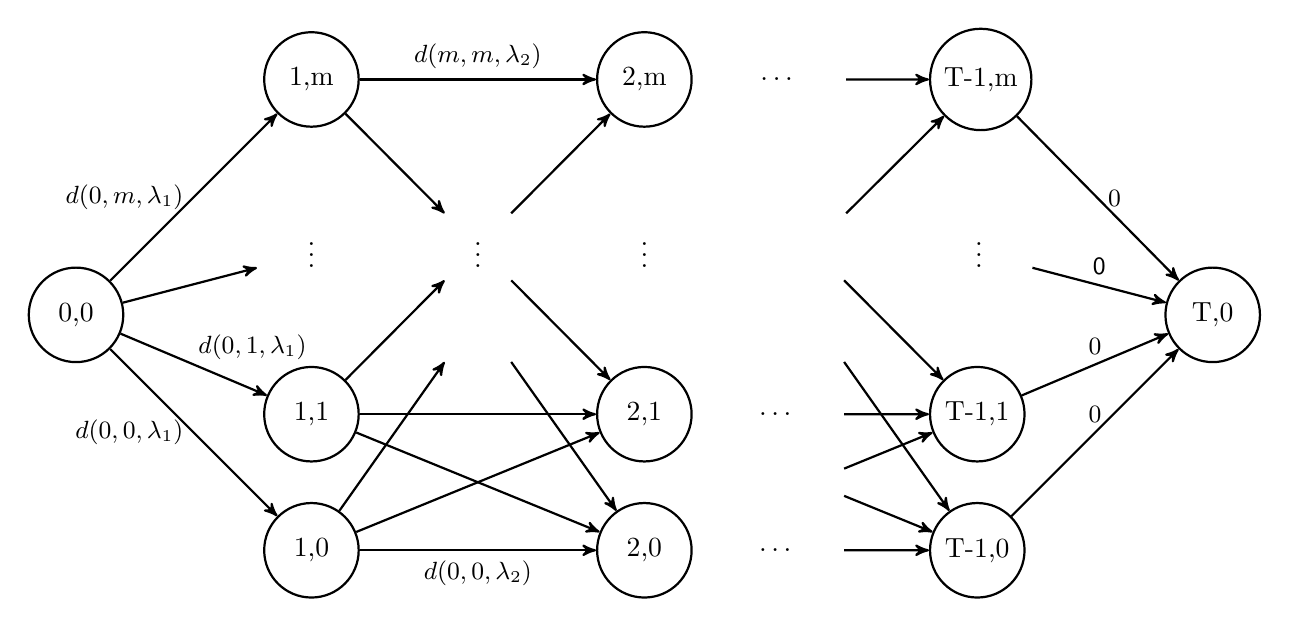
\begin{tikzpicture}[->,>=stealth',auto,node distance=3cm,thick,node/.style={minimum size=1.2cm,circle,draw}]

  \node[node] (1) {0,0};
  \node[node] (4) [below right =of 1] {1,0};
  \node[node] (3) [above =0.5cm of 4] {1,1};
  \node[node] (2) [above right=of 1] {1,m};
  \node[node] (6) [right =of 3] {2,1};
  \node[node] (5) [right =of 2] {2,m};
  \node[node] (7) [right =of 4] {2,0};
  \node[node] (9) [right =of 6] {T-1,1};
  \node[node] (8) [right =of 5] {T-1,m};
  \node[node] (10) [right =of 7] {T-1,0};
  \node[node] (11) [above right =of 10] {T,0};

  \node at ($(5)!.4!(8)$) {\ldots};
  \node at ($(6)!.4!(9)$) {\ldots};
  \node at ($(7)!.4!(10)$) {\ldots};

  \node at ($(2)!.5!(3)$) {\vdots};
  \node at ($(2)!.5!(6)$) {\vdots};
  \node at ($(5)!.5!(6)$) {\vdots};
  \node at ($(8)!.5!(9)$) {\vdots};

  \path[every node/.style={font=\sffamily\small}]
    (1) edge node[left] {$d(0,m,\lambda_1)$} (2)
	edge node[above right=-0.1cm] {$d(0,1,\lambda_1)$} (3)
	edge node[left] {$d(0,0,\lambda_1)$} (4)
    (2) edge node[above] {$d(m,m,\lambda_2)$} (5)
    (3) edge (6)
	edge (7)
    (4) edge (6)
	edge node[below] {$d(0,0,\lambda_2)$} (7)
    (8) edge node[right] {$0$} (11)
    (9) edge node[above] {$0$} (11)
    (10) edge node[above] {$0$} (11);

   \path [->,draw,thick] (1) to ($(1)!.2!(8)$);
   \path [->,draw,thick] (2) to ($(2)!.4!(6)$);
   \path [->,draw,thick] (4) to ($(4)!.4!(5)$);
   \path [->,draw,thick] (3) to ($(3)!.4!(5)$);

   \path [->,draw,thick] ($(3)!.6!(5)$) to (5);
   \path [->,draw,thick] ($(2)!.6!(6)$) to (6);
   \path [->,draw,thick] ($(2)!.6!(7)$) to (7);

   \path [->,draw,thick] ($(6)!.6!(8)$) to (8);
   \path [->,draw,thick] ($(5)!.6!(8)$) to (8);

   \path [->,draw,thick] ($(5)!.6!(9)$) to (9);
   \path [->,draw,thick] ($(6)!.6!(9)$) to (9);
   \path [->,draw,thick] ($(7)!.6!(9)$) to (9);

   \path [->,draw,thick] ($(5)!.6!(10)$) to (10);
   \path [->,draw,thick] ($(6)!.6!(10)$) to (10);
   \path [->,draw,thick] ($(7)!.6!(10)$) to (10);

   \path[every node/.style={font=\sffamily\small}] [->,draw,thick] ($(2)!.8!(11)$) -- node[above] {0} ++ (11);

\end{tikzpicture}
\caption{Graph for optimal schedule algorithm.}
\end{figure}
\begin{remark} 
	All edges from $(t,i)$ to $(t+1,j)$ have weight $d(i,j,\lambda_{t+1})$
\end{remark}

\begin{prop}
	Any given optimal schedule $\mx$ corresponds to a shortest path $P$ from $(0,0)$ to $(T,0)$ with $costs(\mx)=costs(P)$ and vice versa.
\end{prop} 
\begin{proof}
$ $
\begin{itemize}
	\item[``$\Rightarrow$'':] We construct a feasible path in our graph from $\mx$ as follows:
\begin{align*}
	\text{First set}&&e_t&\coloneqq\Bigl(\bigl(t,\mx(t)\bigr),\bigl(t+1,\mx(t+1)\bigr)\Bigr),&\forall t\in\fromto{0}{T-1}\\
	\text{then set}&&P&\coloneqq(e_0,\ldots,e_{T-1})
\end{align*}
As each edge $e_t$ in our graph has weight $d\bigl(\mx(t-1),\mx(t),\lambda_{t}\bigr)$, it corresponds to the costs of switching from $\mx(t-1)$ to $\mx(t)$ servers and processing $\lambda_{t}$ with $\mx(t)$ active servers. Hence, it directly follows that $P$ is a shortest path of the graph with $costs(P)=costs(\mx)$.
	\item[``$\Leftarrow$'':] Let $P=\bigl((0,0)=v_0,\ldots,v_T=(T,0)\bigr)$ with $v_t\in\bigl\{(t,i)\mid 0\le i\le m\bigr\}$ be a shortest path of the graph.\\ 
	We can construct an optimal schedule from $P$ by setting $\mx\coloneqq\bigl(v_0(1),\ldots,v_T(1)\bigr)$\\
	By definition~\eqref{fct:c} it is guaranteed that $P$ only traverses edges such that there are enough active servers $\forall t\in[T]$. Therefore, the created schedule is feasible. Its optimality directly follows from the definition of the edges' weights and so does the equality $costs(\mx)=costs(P)$.
\end{itemize}
\end{proof}

\subsection{A pseudo-polynomial minimum cost algorithm}
\begin{algorithm}[H]
    \caption{Calculate costs for $m$ homogeneous servers}
    \begin{algorithmic}[1]
        \Require{Convex cost function $f$, $\lambda_0=\lambda_T=0$, $\forall t\in[T-1]:\lambda_t\in[0,m]$}
   \Function{schedule}{$m,T,\beta,\lambda_1,\ldots,\lambda_{T-1}$}
	\If{$T<2$} \Return
	\EndIf
	\Blet{$p[2\ldots T-1,m]$ and $M[1\ldots T-1,m]$}{new arrays}
	\For{$j \gets 0 \textrm{ to } m$}
		\Let{$M[1,j]$}{$d(0,j,\lambda_1)$}
	\EndFor
	\For{$t \gets 1 \textrm{ to } T-2$}
		\For{$j \gets 0 \textrm{ to } m$}
			\Let{$opt$}{$\infty$}
			\For{$i \gets 0 \textrm{ to } m$}
				\Let{$M[t+1,j]$}{$M[t,i]+d(i,j,\lambda_{t+1})$}
				\If{$M[t+1,j]<opt$}
					\Let{$opt$}{$M[t+1,j]$}
					\Let{$p[t+1,j]$}{$i$}
				\EndIf
			\EndFor
			\Let{$M[t+1,j]$}{$opt$}
		\EndFor
	\EndFor
	\State \Return{$p$ and $M$}
  \EndFunction
  \end{algorithmic}
\end{algorithm}
\begin{algorithm}[H]
    \caption{Extract schedule for $m$ homogeneous servers}
    \begin{algorithmic}[1]
   \Function{Extract}{$m,p,M,T$}
	\Blet{$x[0\ldots T]$}{a new array}
	\Let{$x[0]$}{$x[T]\leftarrow 0$}
	\If{$T<2$} \Return $x$ \Comment{Trivial solution}
	\EndIf
	\Let{$x[T-1]$}{$\underset{0\le i\le m}{arg\ min}\{M[T-1,i]\}$}
	\For{$t \gets T-2 \textrm{ to } 1$}
		\Let{$x[t]$}{$p[t+1,x[t+1]]$}
	\EndFor
	\State \Return{$x$}
  \EndFunction
  \end{algorithmic}
\end{algorithm}

\subsubsection{Runtime analysis}
The algorithm visits every vertex and every edge of the graph exactly once. As the number of vertices is bounded by $\mathcal{O}(Tm)$ and the number of edges is bounded by $\mathcal{O}(Tm^2)$ the running time is given by:
\begin{equation*}
	\mathcal{O}(Tm+Tm^2)=\mathcal{O}(Tm^2)
\end{equation*}
As we need $\log_2(m)$ bits to encode m, the running time is polynomial in the numeric value of the input but exponential in the length of the input. Hence, the algorithm is pseudo-polynomial.

\subsubsection{A memory optimized algorithm}
TODO: use only array with size 2m

\section{A polynomial $4$-approximation algorithm for monotonically increasing convex f}
We consider a modification of the problem discussed in chapter~\ref{sec:opt}. Assuming that f is convex and monotonically increasing, we can modify our algorithm to obtain a polynomial time $4$-approximation algorithm.

\subsection{Graph for a $4$-optimal schedule}
We modify our graph from chapter~\ref{sec:optgraph} to the reduce the number of vertices. For this, we stop adding m vertices for each timestep, but use vertices that approximate the number of active servers instead. First, let $b\coloneqq\lceil\log_2(m)\rceil$. We add vertices $(t,0)$ and $(t,2^i),\forall t\in[T-1],0\le i\le b$. All edges and weights are added analogous to chapter~\ref{sec:optgraph}.
\begin{figure}[H]
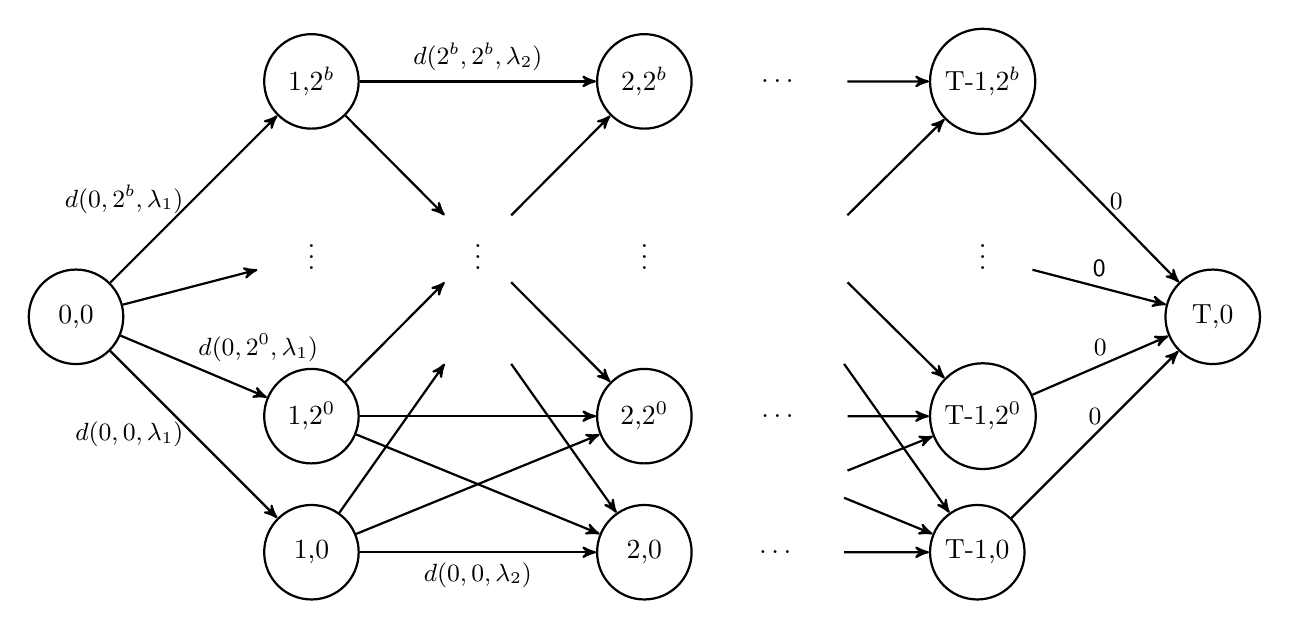
\begin{tikzpicture}[->,>=stealth',auto,node distance=3cm,thick,node/.style={minimum size=1.2cm,circle,draw}]

  \node[node] (1) {0,0};
  \node[node] (4) [below right =of 1] {1,0};
  \node[node] (3) [above =0.5cm of 4] {1,$2^0$};
  \node[node] (2) [above right=of 1] {1,$2^b$};
  \node[node] (6) [right =of 3] {2,$2^0$};
  \node[node] (5) [right =of 2] {2,$2^b$};
  \node[node] (7) [right =of 4] {2,0};
  \node[node] (9) [right =of 6] {T-1,$2^0$};
  \node[node] (8) [right =of 5] {T-1,$2^b$};
  \node[node] (10) [right =of 7] {T-1,0};
  \node[node] (11) [above right =of 10] {T,0};

  \node at ($(5)!.4!(8)$) {\ldots};
  \node at ($(6)!.4!(9)$) {\ldots};
  \node at ($(7)!.4!(10)$) {\ldots};

  \node at ($(2)!.5!(3)$) {\vdots};
  \node at ($(2)!.5!(6)$) {\vdots};
  \node at ($(5)!.5!(6)$) {\vdots};
  \node at ($(8)!.5!(9)$) {\vdots};

  \path[every node/.style={font=\sffamily\small}]
    (1) edge node[left] {$d(0,2^b,\lambda_1)$} (2)
	edge node[above right=-0.1cm] {$d(0,2^0,\lambda_1)$} (3)
	edge node[left] {$d(0,0,\lambda_1)$} (4)
    (2) edge node[above] {$d(2^b,2^b,\lambda_2)$} (5)
    (3) edge (6)
	edge (7)
    (4) edge (6)
	edge node[below] {$d(0,0,\lambda_2)$} (7)
    (8) edge node[right] {$0$} (11)
    (9) edge node[above] {$0$} (11)
    (10) edge node[above] {$0$} (11);

   \path [->,draw,thick] (1) to ($(1)!.2!(8)$);
   \path [->,draw,thick] (2) to ($(2)!.4!(6)$);
   \path [->,draw,thick] (4) to ($(4)!.4!(5)$);
   \path [->,draw,thick] (3) to ($(3)!.4!(5)$);

   \path [->,draw,thick] ($(3)!.6!(5)$) to (5);
   \path [->,draw,thick] ($(2)!.6!(6)$) to (6);
   \path [->,draw,thick] ($(2)!.6!(7)$) to (7);

   \path [->,draw,thick] ($(6)!.6!(8)$) to (8);
   \path [->,draw,thick] ($(5)!.6!(8)$) to (8);

   \path [->,draw,thick] ($(5)!.6!(9)$) to (9);
   \path [->,draw,thick] ($(6)!.6!(9)$) to (9);
   \path [->,draw,thick] ($(7)!.6!(9)$) to (9);

   \path [->,draw,thick] ($(5)!.6!(10)$) to (10);
   \path [->,draw,thick] ($(6)!.6!(10)$) to (10);
   \path [->,draw,thick] ($(7)!.6!(10)$) to (10);

   \path[every node/.style={font=\sffamily\small}] [->,draw,thick] ($(2)!.8!(11)$) -- node[above] {0} ++ (11);

\end{tikzpicture}
\caption{Graph for a $4$-approximation algorithm}
\end{figure}

\begin{defn}
Let $\mx=(x_0,\ldots,x_T)$ be a schedule and $t>0$.\\
We say that $\mx$ changes its \textbf{state} at time t if
\begin{equation*}
	x_t\neq x_{t-1}
\end{equation*}
and that $\mx$ changes its \textbf{2-state} at time t if
\begin{equation*}
	x_t=0\text{\quad or\quad}x_t\notin\bigl(2^{\lfloor \log_2(x_{t-1})\rfloor},2^{\lceil \log_2(x_{t-1})\rceil}\bigr)
\end{equation*}
\end{defn}
\begin{prop}
$ $
\begin{enumerate}
	\item\label{prop:2opt} Any given optimal schedule $\mx$ can be transformed to a $4$-optimal schedule $\mx'$ which corresponds to a path $P$ from $(0,0)$ to $(T,0)$ with $costs(\mx')=costs(P)$.
	\item Any shortest path $P$ from $(0,0)$ to $(T,0)$ corresponds to a $4$-optimal schedule $\mx$ with $costs(P)=costs(\mx)$.
\end{enumerate}
\end{prop}
\begin{proof}
$ $
\begin{enumerate}
	\item Assume we have an optimal schedule identified by $\mx=(x_0,\ldots,x_T)$. For $0\le t<T$ we inductively set:
\begin{equation}
	x'_0\coloneqq 0,\qquad
	x'_{t+1}\coloneqq 
	\begin{cases}
		\min\bigl\{2^{\lfloor \log_2(2x_{t+1})\rfloor},2^b\bigr\}, & \text{if $0<x_t\le x_{t+1}$}\\
		2^{\lceil \log_2(2x_{t+1})\rceil}, & \text{if $0<x_{t+1}<x_t$ and $x'_{t}\ge4x_{t+1}$}\\
		x'_t, & \text{if $0<x_{t+1}<x_t$ and $x'_{t}<4x_{t+1}$}\\
		\		   0, & \text{otherwise}
	\end{cases} \label{def:chi_prime}
\end{equation}
Then let $\mx'\coloneqq(x'_0,\ldots,x'_T)$ be the modified sequence of active servers. Notice that \makebox{$x_t\le x'_t\le 4x_t$} holds as $x'_t$ is at most the smallest power of two larger than $2x_t$ which implies that $\mx'$ is feasible.\\
We can now construct a feasible path in our graph from $\mathcal{X'}$ as follows:
\begin{align*}
	\text{First set}&&e_t&\coloneqq\Bigl(\bigl(t,\mx'(t)\bigr),\bigl(t+1,\mx'(t+1)\bigr)\Bigr),&\forall t\in\fromto{0}{T-1}\\
	\text{then set}&&P&\coloneqq(e_0,\ldots,e_{T-1})
\end{align*}
By the definition of the edges' weights it follows that $costs(\mx')=costs(P)$.\\
Next, let $(t_0=0,t_1,\ldots,t_n=0)$ be the sequence of times where the optimal schedule $\mx$ changes its 2-state. Notice that the modified schedule $\mx'$ changes its state only at times $t_i$ and that $2x_{t_i}\le x'_{t_i}$ holds (TODO: only if not discrete but continous time steps). This can be seen exemplarily in figure~\ref{fig:adaption-schedule} by obvserving that $\mx'$ changes its state only if $\mx$ crosses or touches a bordering power of two.
\begin{figure}[H]
\centering
\scalebox{0.7}{
\subfloat{
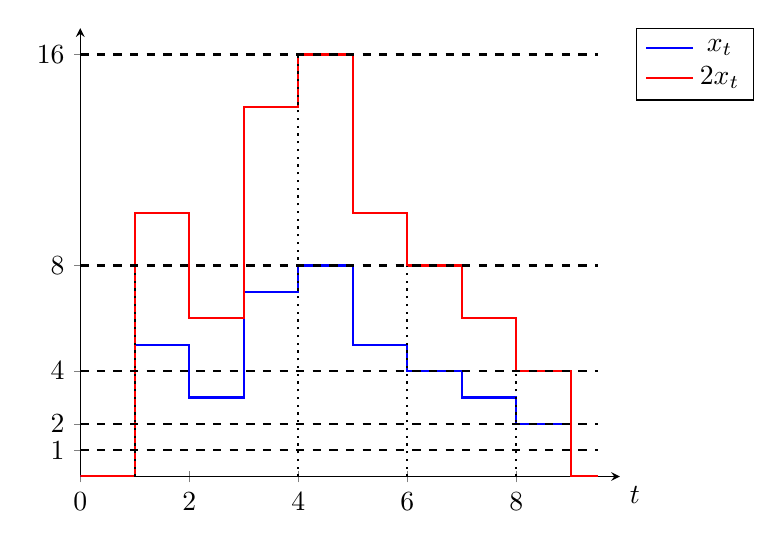
\begin{tikzpicture}
	\begin{axis}[%
	    ,xlabel=$t$
	    ,axis x line = bottom,axis y line = left
	    ,ytick={1,2,4,8,16}
	    ,ymax=17 % or enlarge y limits=upper
	    ,xmax=9.9
	    ,legend pos=outer north east
	    ]
	\addplot+[const plot, no marks, thick, color=blue] coordinates {(0,0) (1,5) (2,3) (3,7) (4,8) (5,5) (6,4) (7,3) (8,2) (9,0) (9.5,0)};
	\addplot+[const plot, no marks, thick, color=red] coordinates {(0,0) (1,10) (2,6) (3,14) (4,16) (5,10) (6,8) (7,6) (8,4) (9,0) (9.5,0)};
	\addplot+[const plot, no marks, thick, dotted, color=black] coordinates {(1,0) (1,8)};
	\addplot+[const plot, no marks, thick, dotted, color=black] coordinates {(4,0) (4,16)};
	\addplot+[const plot, no marks, thick, dotted, color=black] coordinates {(6,0) (6,8)};
	\addplot+[const plot, no marks, thick, dotted, color=black] coordinates {(8,0) (8,4)};
	\addplot+[const plot, no marks, thick, dashed, color=black] coordinates {(0,1) (9.5,1)};
	\addplot+[const plot, no marks, thick, dashed, color=black] coordinates {(0,2) (9.5,2)};
	\addplot+[const plot, no marks, thick, dashed, color=black] coordinates {(0,4) (9.5,4)};
	\addplot+[const plot, no marks, thick, dashed, color=black] coordinates {(0,8) (9.5,8)};
	\addplot+[const plot, no marks, thick, dashed, color=black] coordinates {(0,16) (9.5,16)};
	\addlegendentry{$x_t$}
	\addlegendentry{$2x_t$}
	\end{axis}
\end{tikzpicture}}}
\qquad
\scalebox{0.7}{
\subfloat{
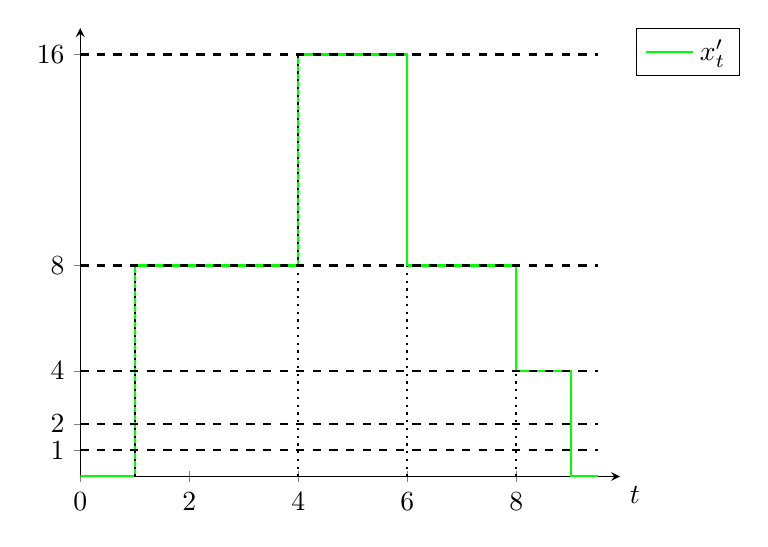
\begin{tikzpicture}
	\begin{axis}[%
	    ,xlabel=$t$
	    ,axis x line = bottom,axis y line = left
	    ,ytick={1,2,4,8,16}
	    ,ymax=17 % or enlarge y limits=upper
	    ,xmax=9.9
	    ,legend pos=outer north east
	    ]
	\addplot+[const plot, no marks, thick, color=green] coordinates {(0,0) (1,8) (2,8) (3,8) (4,16) (5,16) (6,8) (7,8) (8,4) (9,0) (9.5,0)};
	\addplot+[const plot, no marks, thick, dotted, color=black] coordinates {(1,0) (1,8)};
	\addplot+[const plot, no marks, thick, dotted, color=black] coordinates {(4,0) (4,16)};
	\addplot+[const plot, no marks, thick, dotted, color=black] coordinates {(6,0) (6,8)};
	\addplot+[const plot, no marks, thick, dotted, color=black] coordinates {(8,0) (8,4)};
	\addplot+[const plot, no marks, thick, dashed, color=black] coordinates {(0,1) (9.5,1)};
	\addplot+[const plot, no marks, thick, dashed, color=black] coordinates {(0,2) (9.5,2)};
	\addplot+[const plot, no marks, thick, dashed, color=black] coordinates {(0,4) (9.5,4)};
	\addplot+[const plot, no marks, thick, dashed, color=black] coordinates {(0,8) (9.5,8)};
	\addplot+[const plot, no marks, thick, dashed, color=black] coordinates {(0,16) (9.5,16)};
	\addlegendentry{$x'_t$}
	\end{axis}
\end{tikzpicture}}}
 	\caption{Adaption of an optimal schedule}
	\label{fig:adaption-schedule}
\end{figure}
	For this reason, we now only have to consider the fraction of costs of $\mx'$ and $\mx$ between time steps $t_{i-1}$ and $t_i$
	\begin{equation}
		\frac{costs(\mx',t_{i-1},t_i)}{costs(\mx,t_{i-1},t_i)}\label{eq:frac_chi_prime}
	\end{equation}
	For $x_{t_i}=0$ it follows from \eqref{eq:costs_chi_t_t_prime} that $costs(\mx',t_{i-1},t_i)=costs(\mx,t_{i-1},t_i)=0$. Hence, we can restrict ourselves to $0<t_i<T$ with $x_{t_i}\neq 0$.
	The costs incurred by $\mx'$ are given by
	\begin{align}
		&&costs(\mx',t_{i-1},t_i)&=\beta\max\{0,x'_{t_i}-x'_{t_{i-1}}\}+x'_{t_i}f(\lambda_{t_i}/x'_{t_i})&\text{by \eqref{eq:costs_chi_t_t_prime}}\nonumber\\
		&&&\le\beta\max\{0,x'_{t_i}-x'_{t_{i-1}}\}+4x_{t_i}f(\lambda_{t_i}/x'_{t_i})&\text{by \eqref{def:chi_prime}}\nonumber\\
		&&&\le\beta\max\{0,x'_{t_i}-x'_{t_{i-1}}\}+4x_{t_i}f(\lambda_{t_i}/x_{t_i})&\text{f monotonically increasing}\nonumber\\
		\implies&&costs(\mx',t_{i-1},t_i)&\le\beta\max\{0,x'_{t_i}-x'_{t_{i-1}}\}+4x_{t_i}f(\lambda_{t_i}/x_{t_i})\label{eq:est_chi_prime}
	\end{align}
	and the costs of $\mx$ by
	\begin{equation}
		costs(\mx,t_{i-1},t_i)=\beta\max\{0,x_{t_i}-x_{t_{i-1}}\}+x_{t_i}f(\lambda_{t_i}/x_{t_i})\label{eq:optcosts}
	\end{equation}
	W.l.o.g.\ we may assume $x_{t_i}f(\lambda_{t_i}/x_{t_i})>0$, otherwise the claim follows trivially. (TODO: is it really trivial?)
	\begin{enumerate}[(i)]
		\item\label{pr:4appr_1} \underline{$x_{t_i}\le x_{t_{i-1}}$:}
			From~\eqref{def:chi_prime} it follows that $x'_{t_i}\le x'_{t_{i-1}}$. Thus, we can simplify~\eqref{eq:frac_chi_prime}:
		\begin{align*}
			\frac{costs(\mx',t_{i-1},t_i)}{costs(\mx,t_{i-1},t_i)}&\le\frac{\beta\max\{0,x'_{t_i}-x'_{t_{i-1}}\}+4x_{t_i}f(\lambda_{t_i}/x_{t_i})}{\beta\max\{0,x_{t_i}-x_{t_{i-1}}\}+x_{t_i}f(\lambda_{t_i}/x_{t_i})}&\text{by \eqref{eq:est_chi_prime},\eqref{eq:optcosts}}\\
			&=\frac{4x_{t_i}f(\lambda_{t_i}/x_{t_i})}{x_{t_i}f(\lambda_{t_i}/x_{t_i})}&\text{($x_{t_i}\le x_{t_{i-1}}$ and $x'_{t_i}\le x'_{t_{i-1}}$)}\\
			&=4
		\end{align*}
		\item\label{pr:4appr_2} \underline{$x_{t_i}>x_{t_{i-1}}$:}
		From (\ref{def:chi_prime}) it follows that $x'_{t_i}\ge x'_{t_{i-1}}$. Thus, we can simplify~(\ref{eq:frac_chi_prime}):
		\begin{align*}
			\frac{costs(\mx',t_{i-1},t_i)}{costs(\mx,t_{i-1},t_i)}&\le\frac{\beta\max\{0,x'_{t_i}-x'_{t_{i-1}}\}+4x_{t_i}f(\lambda_{t_i}/x_{t_i})}{\beta\max\{0,x_{t_i}-x_{t_{i-1}}\}+x_{t_i}f(\lambda_{t_i}/x_{t_i})}&\text{by \eqref{eq:est_chi_prime},\eqref{eq:optcosts}}\\
			&=\frac{\beta(x'_{t_i}-x'_{t_{i-1}})+4x_{t_i}f(\lambda_{t_i}/x_{t_i})}{\beta(x_{t_i}-x_{t_{i-1}})+x_{t_i}f(\lambda_{t_i}/x_{t_i})}&\text{($x_{t_i}>x_{t_{i-1}}$ and $x'_{t_i}\ge x'_{t_{i-1}}$)}\\
			&=\frac{\beta(\min\bigl\{2^{\lfloor \log_2(2x_{t_i})\rfloor},2^b\bigr\}-x'_{t_{i-1}})+4x_{t_i}f(\lambda_{t_i}/x_{t_i})}{\beta(x_{t_i}-x_{t_{i-1}})+x_{t_i}f(\lambda_{t_i}/x_{t_i})}&\text{by \eqref{def:chi_prime}}\\
			&\le\frac{\beta(2^{\lfloor \log_2(2x_{t_i})\rfloor}-x'_{t_{i-1}})+4x_{t_i}f(\lambda_{t_i}/x_{t_i})}{\beta(x_{t_i}-x_{t_{i-1}})+x_{t_i}f(\lambda_{t_i}/x_{t_i})}\\
			&\le\frac{\beta(2x_{t_i}-x'_{t_{i-1}})+4x_{t_i}f(\lambda_{t_i}/x_{t_i})}{\beta(x_{t_i}-x_{t_{i-1}})+x_{t_i}f(\lambda_{t_i}/x_{t_i})}\\
			&\le\frac{\beta(2x_{t_i}-2x_{t_{i-1}})+4x_{t_i}f(\lambda_{t_i}/x_{t_i})}{\beta(x_{t_i}-x_{t_{i-1}})+x_{t_i}f(\lambda_{t_i}/x_{t_i})}&\text{by ($2x_{t_{i-1}}\le x'_{t_{i-1}}$)}\\
			&\le4\ \frac{\frac{1}{2}\beta(x_{t_i}-x_{t_{i-1}})+x_{t_i}f(\lambda_{t_i}/x_{t_i})}{\ \ \beta(x_{t_i}-x_{t_{i-1}})+x_{t_i}f(\lambda_{t_i}/x_{t_i})}\\
			&\le4
		\end{align*}
	\end{enumerate}
	From~(\hyperref[pr:4appr_1]{i}) and~(\hyperref[pr:4appr_2]{ii}) it follows:
	\begin{equation*}
		costs(\mx')\le4costs(\mx)
	\end{equation*}
	\item From~\ref{prop:2opt} we obtain that we can construct a $4$-optimal path $P'$ from any optimal schedule. Now, let $P$ be a shortest path. We have $costs(P)\le costs(P')<\infty$, and since every path $P$ with $costs(P)<\infty$ corresponds to a feasible schedule $\mx$ with $costs(P)=costs(\mx)$, $\mx$ must also be at least $4$-optimal.
\end{enumerate}
\end{proof}

\newpage
\bibliographystyle{plain}
\bibliography{sources.bib}
\newpage

\section*{Appendix}
Below, we give an overview of just given definitions and conventions commonly referred to in our paper:
%\scriptsize
%\begin{multicols}{2}
\begin{itemize}
	\item $m\in\mathbb{N}$\ldots number of homogeneous servers
	\item $T\in\mathbb{N}$\ldots number of time slots
	\item $\lambda_1,\ldots,\lambda_{T}\in[0,m]$\ldots arrival rates
	\item $\Lambda\coloneqq(\lambda_1,\ldots,\lambda_T)$\ldots sequence of arrival rates
	\item $\beta\in\mathbb{R}_{\ge 0}$\ldots switching costs of a server
	\item $f:[0,1]\rightarrow\mathbb{R}$\ldots convex operating costs function of a server
	\item $\mathcal{I}\coloneqq(m,T,\Lambda,\beta,f)$\ldots input of problem instance
	\item $\lambda_{i,t}\in[0,1]$\ldots assigned load for server $i$ at time $t$
	\item $\mathcal{L}\coloneqq(\lambda_{0,1},\lambda_{2,1},\ldots,\lambda_{m,1},\lambda_{1,2},\ldots,\lambda_{m,T})$\ldots sequence of assigned loads
	\item $s_{i,t}$\ldots state of server $i$ at time $t$, i.e.\ sleeping (0) or active(1)
	\item $\mathcal{S}\coloneqq(s_{1,1},s_{2,1},\ldots,s_{m,1},s_{1,2},\ldots,s_{m,T})\in\{0,1\}^{m*T}$\ldots sequence of states 
	\item $x_t$\ldots number of active servers at time t
	\item $\mx\coloneqq(x_1,\ldots,x_T)$\ldots sequence of number of active servers
	\item $\lambda_{t}=0$ for all $t\notin[T]$
	\item All servers are powered down at time $t=0$
\end{itemize}
%\end{multicols}
\normalsize

\end{document}
